\chapter{Resultados}

Este capítulo apresenta os resultados da aplicação dos seis LLMs \textit{open-source} sobre as 79 normas brasileiras do \textit{dataset}, nos três experimentos comparativos definidos no capítulo anterior: EN1 (segmentação N1 isolada), EN2 (identificação RASE com N1 de referência) e EN1N2 (\textit{pipeline} encadeado N1$\rightarrow$N2). Todos os números vêm diretamente dos arquivos \texttt{metrics/validate\_*.json}, gerados pela rotina de validação descrita na Seção~3.7. Para cada experimento, o texto traz as médias agregadas por métrica, os resultados detalhados por modelo, os tempos de execução e uma discussão integrada. A Seção~\ref{sec:n3} traz, em separado, os resultados isolados do N3.

\section{Visão Geral dos Experimentos}

A Tabela~\ref{tab:metricas_resultados} resume as médias por métrica nos três experimentos comparativos, agregadas sobre os seis modelos. Dois padrões já saltam aos olhos: as métricas baseadas em \textit{embeddings} (SBERT, BERTimbau, Multilingual e BERTScore) mantêm desempenho consistentemente mais alto, e as lexicais (FuzzyWuzzy, TF-IDF e ROUGE-L) perdem terreno à medida que se sai do EN1 e se entra no EN1N2.

\begin{table}[ht]
\centering
\caption{Médias por métrica nos três experimentos, agregadas sobre os seis modelos.}
\label{tab:metricas_resultados}
\small
\begin{tabular}{lccc}
\hline
Métrica       & EN1   & EN2   & EN1N2 \\
\hline
FuzzyWuzzy    & 0{,}475 & 0{,}461 & 0{,}464 \\
TF-IDF        & 0{,}636 & 0{,}312 & 0{,}417 \\
SBERT         & 0{,}801 & 0{,}490 & 0{,}594 \\
BERTimbau     & 0{,}816 & 0{,}542 & 0{,}631 \\
Multilingual  & 0{,}850 & 0{,}595 & 0{,}679 \\
WMD\_ft       & 0{,}716 & 0{,}580 & 0{,}625 \\
WMD\_nilc     & 0{,}688 & 0{,}546 & 0{,}595 \\
BERTScore     & 0{,}866 & 0{,}753 & 0{,}790 \\
ROUGE-L       & 0{,}599 & 0{,}308 & 0{,}404 \\
\hline
Acurácia      & 0{,}475 & 0{,}273 & --- \\
Precisão      & 0{,}545 & 0{,}202 & --- \\
Revocação     & 0{,}774 & 0{,}198 & --- \\
F1-score      & 0{,}631 & 0{,}197 & --- \\
\hline
\end{tabular}
\end{table}

As métricas semânticas (SBERT, BERTimbau e Multilingual), junto do BERTScore, preservaram melhor o valor agregado ao longo dos três experimentos --- são mais robustas a variações de superfície. As lexicais e o ROUGE-L sofrem com a reformulação produzida pelos LLMs. No N3 (estruturação JSON), as métricas de similaridade textual seguem altas (ver Seção~\ref{sec:n3}), mas as métricas de classificação por correspondência exata expõem dificuldades sistemáticas na produção dos campos estruturados.

\section{Resultados por Experimento}

\subsection{EN1 --- Segmentação N1}

No EN1, a comparação foi entre as regras N1 geradas pelos LLMs e o N1 de referência. As métricas semânticas ficaram bem acima das lexicais --- Multilingual~0{,}850, BERTimbau~0{,}816 e SBERT~0{,}801, contra TF-IDF~0{,}636 e FuzzyWuzzy~0{,}475 ---, o que indica que a segmentação tolera reformulação lexical quando o sentido é preservado. O \textbf{Dolphin} dominou: liderou em \textit{todas} as nove métricas de similaridade e em três das quatro de classificação, com o melhor desempenho isolado do experimento. Os números detalhados estão na Tabela~\ref{tab:resultados_en1}.

\begin{table}[ht]
\centering
\caption{Resultados por modelo em EN1 (similaridade e classificação).}
\label{tab:resultados_en1}
\scriptsize
\begin{tabular}{lccccccccc}
\hline
Modelo & FW & TF-IDF & SBERT & BERTimbau & Multi. & WMD\_ft & WMD\_nilc & BERTScore & ROUGE-L \\
\hline
Alpaca  & 0{,}473 & 0{,}561 & 0{,}748 & 0{,}762 & 0{,}803 & 0{,}694 & 0{,}664 & 0{,}841 & 0{,}540 \\
Dolphin & \textbf{0{,}641} & \textbf{0{,}756} & \textbf{0{,}873} & \textbf{0{,}891} & \textbf{0{,}913} & \textbf{0{,}774} & \textbf{0{,}751} & \textbf{0{,}905} & \textbf{0{,}703} \\
Gemma   & 0{,}412 & 0{,}695 & 0{,}842 & 0{,}850 & 0{,}885 & 0{,}726 & 0{,}699 & 0{,}883 & 0{,}648 \\
Llama   & 0{,}422 & 0{,}672 & 0{,}835 & 0{,}844 & 0{,}873 & 0{,}711 & 0{,}684 & 0{,}871 & 0{,}605 \\
Mistral & 0{,}534 & 0{,}704 & 0{,}842 & 0{,}874 & 0{,}899 & 0{,}726 & 0{,}699 & 0{,}888 & 0{,}651 \\
Qwen    & 0{,}367 & 0{,}429 & 0{,}668 & 0{,}673 & 0{,}726 & 0{,}663 & 0{,}632 & 0{,}808 & 0{,}448 \\
\hline
\multicolumn{10}{c}{Métricas de classificação (Acurácia / Precisão / Revocação / F1)} \\
\hline
Alpaca  & \multicolumn{9}{l}{0{,}419 / 0{,}512 / 0{,}699 / 0{,}591} \\
Dolphin & \multicolumn{9}{l}{\textbf{0{,}676} / \textbf{0{,}812} / 0{,}801 / \textbf{0{,}806}} \\
Gemma   & \multicolumn{9}{l}{0{,}466 / 0{,}486 / \textbf{0{,}917} / 0{,}636} \\
Llama   & \multicolumn{9}{l}{0{,}446 / 0{,}479 / 0{,}865 / 0{,}616} \\
Mistral & \multicolumn{9}{l}{0{,}610 / 0{,}670 / 0{,}872 / 0{,}758} \\
Qwen    & \multicolumn{9}{l}{0{,}235 / 0{,}311 / 0{,}487 / 0{,}380} \\
\hline
\end{tabular}
\end{table}

A Figura~\ref{img:4.2.1} apresenta o comparativo visual entre os seis modelos nas nove métricas de similaridade em EN1.

\begin{figure}[ht]
\centering
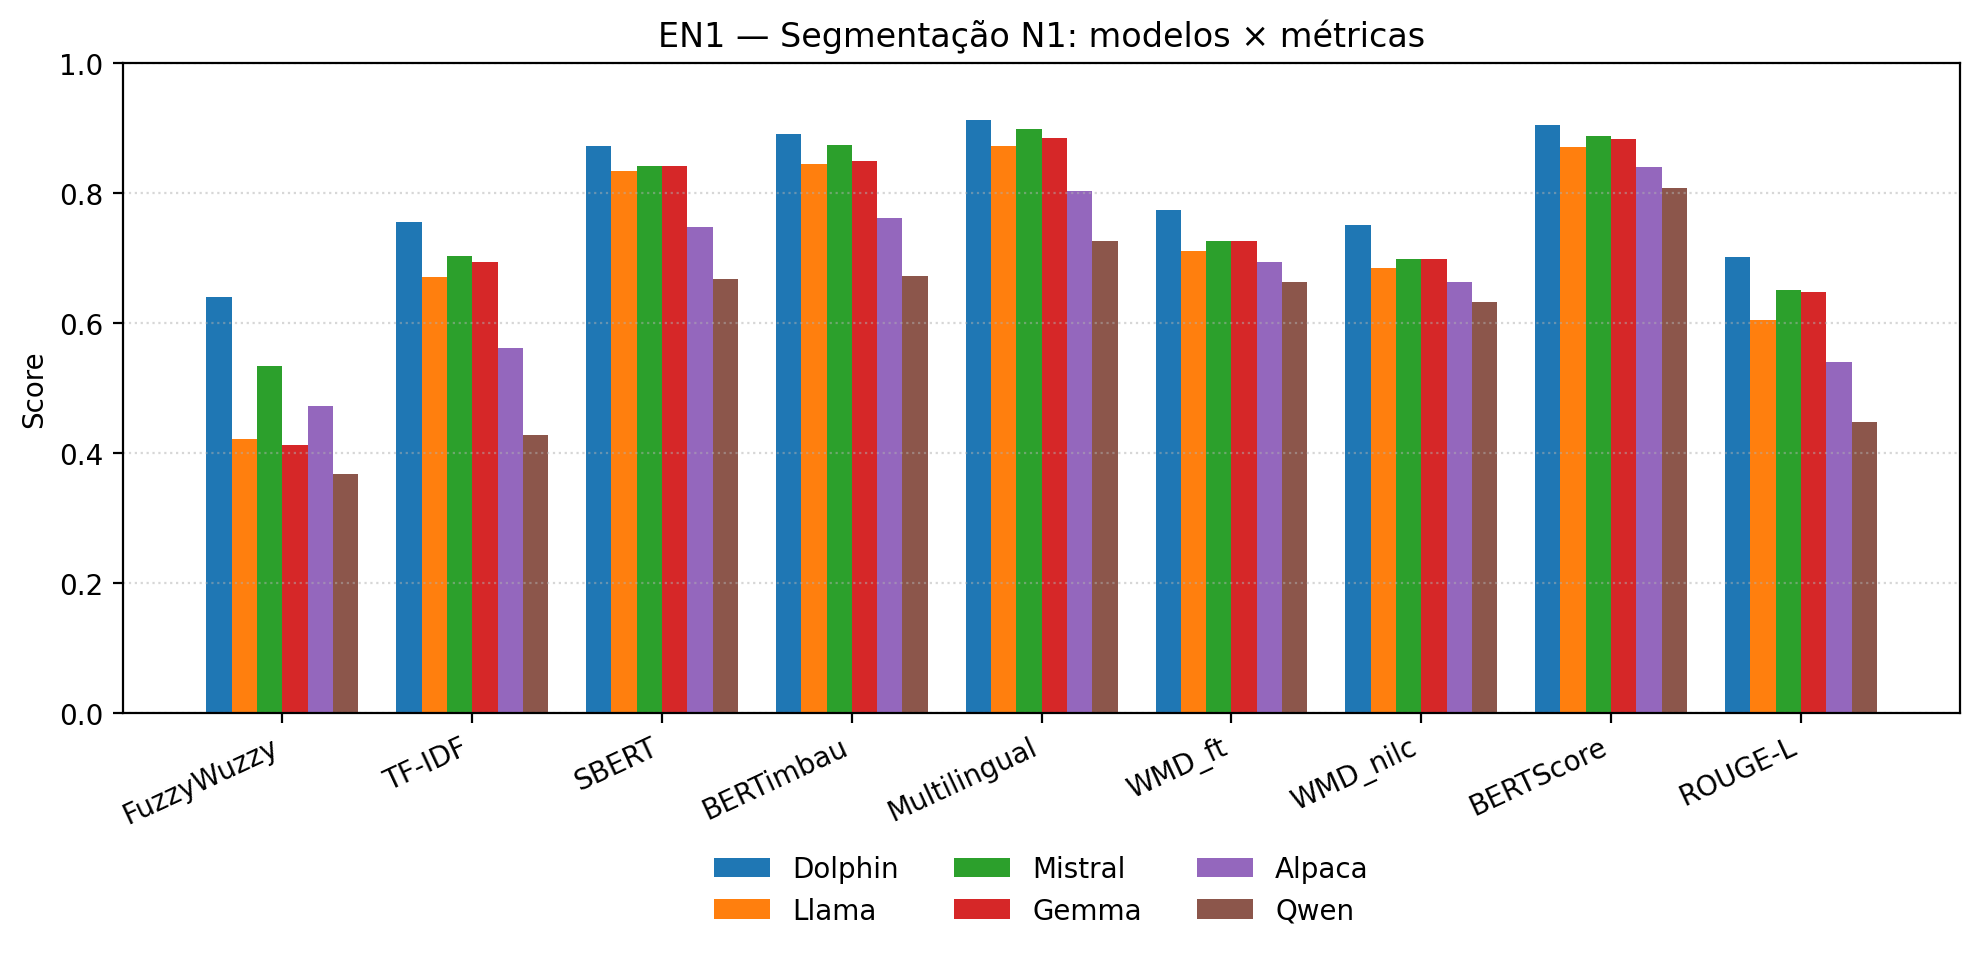
\includegraphics[width=0.95\linewidth]{Imagens/4.2.1-resultados-en1-barras.png}
\caption{Comparativo modelo $\times$ métrica em EN1.}
\label{img:4.2.1}
\end{figure}

\subsection{EN2 --- Identificação dos Operadores RASE}

O EN2 mediu a identificação e a estruturação dos operadores RASE a partir do N1 de referência. As médias caíram em relação ao EN1 (SBERT~0{,}490; Multilingual~0{,}595), o que reflete a maior dificuldade da formalização estruturada. As métricas de classificação caem ainda mais (F1 macro~0{,}197): os modelos têm dificuldade real em distinguir Seleção e Exceção. O \textbf{Llama} lidera nas métricas semânticas e lexicais; o \textbf{Dolphin} fica com a melhor F1 macro (0{,}286). Os números detalhados estão na Tabela~\ref{tab:resultados_en2}.

\begin{table}[ht]
\centering
\caption{Resultados por modelo em EN2 (similaridade e classificação macro por operador).}
\label{tab:resultados_en2}
\scriptsize
\begin{tabular}{lccccccccc}
\hline
Modelo & FW & TF-IDF & SBERT & BERTimbau & Multi. & WMD\_ft & WMD\_nilc & BERTScore & ROUGE-L \\
\hline
Alpaca  & 0{,}334 & 0{,}168 & 0{,}386 & 0{,}418 & 0{,}484 & 0{,}522 & 0{,}486 & 0{,}702 & 0{,}172 \\
Dolphin & 0{,}511 & 0{,}423 & 0{,}557 & 0{,}621 & 0{,}665 & \textbf{0{,}620} & \textbf{0{,}589} & 0{,}786 & 0{,}412 \\
Gemma   & 0{,}384 & 0{,}364 & 0{,}520 & 0{,}579 & 0{,}625 & 0{,}608 & 0{,}577 & 0{,}772 & 0{,}350 \\
Llama   & \textbf{0{,}638} & \textbf{0{,}447} & \textbf{0{,}595} & \textbf{0{,}657} & \textbf{0{,}685} & 0{,}617 & 0{,}586 & \textbf{0{,}796} & \textbf{0{,}427} \\
Mistral & 0{,}563 & 0{,}385 & 0{,}575 & 0{,}607 & 0{,}665 & 0{,}607 & 0{,}575 & 0{,}779 & 0{,}377 \\
Qwen    & 0{,}336 & 0{,}083 & 0{,}304 & 0{,}369 & 0{,}444 & 0{,}496 & 0{,}462 & 0{,}684 & 0{,}111 \\
\hline
\multicolumn{10}{c}{Métricas de classificação --- macro (Acurácia / Precisão / Revocação / F1)} \\
\hline
Alpaca  & \multicolumn{9}{l}{0{,}081 / 0{,}103 / 0{,}109 / 0{,}105} \\
Dolphin & \multicolumn{9}{l}{0{,}339 / 0{,}301 / 0{,}276 / \textbf{0{,}286}} \\
Gemma   & \multicolumn{9}{l}{0{,}182 / 0{,}252 / \textbf{0{,}300} / 0{,}265} \\
Llama   & \multicolumn{9}{l}{\textbf{0{,}439} / 0{,}237 / 0{,}250 / 0{,}243} \\
Mistral & \multicolumn{9}{l}{0{,}434 / 0{,}268 / 0{,}214 / 0{,}238} \\
Qwen    & \multicolumn{9}{l}{0{,}160 / 0{,}051 / 0{,}039 / 0{,}044} \\
\hline
\end{tabular}
\end{table}

A Figura~\ref{img:4.2.2} consolida o desempenho dos seis modelos nas nove métricas de similaridade em EN2.

\begin{figure}[ht]
\centering
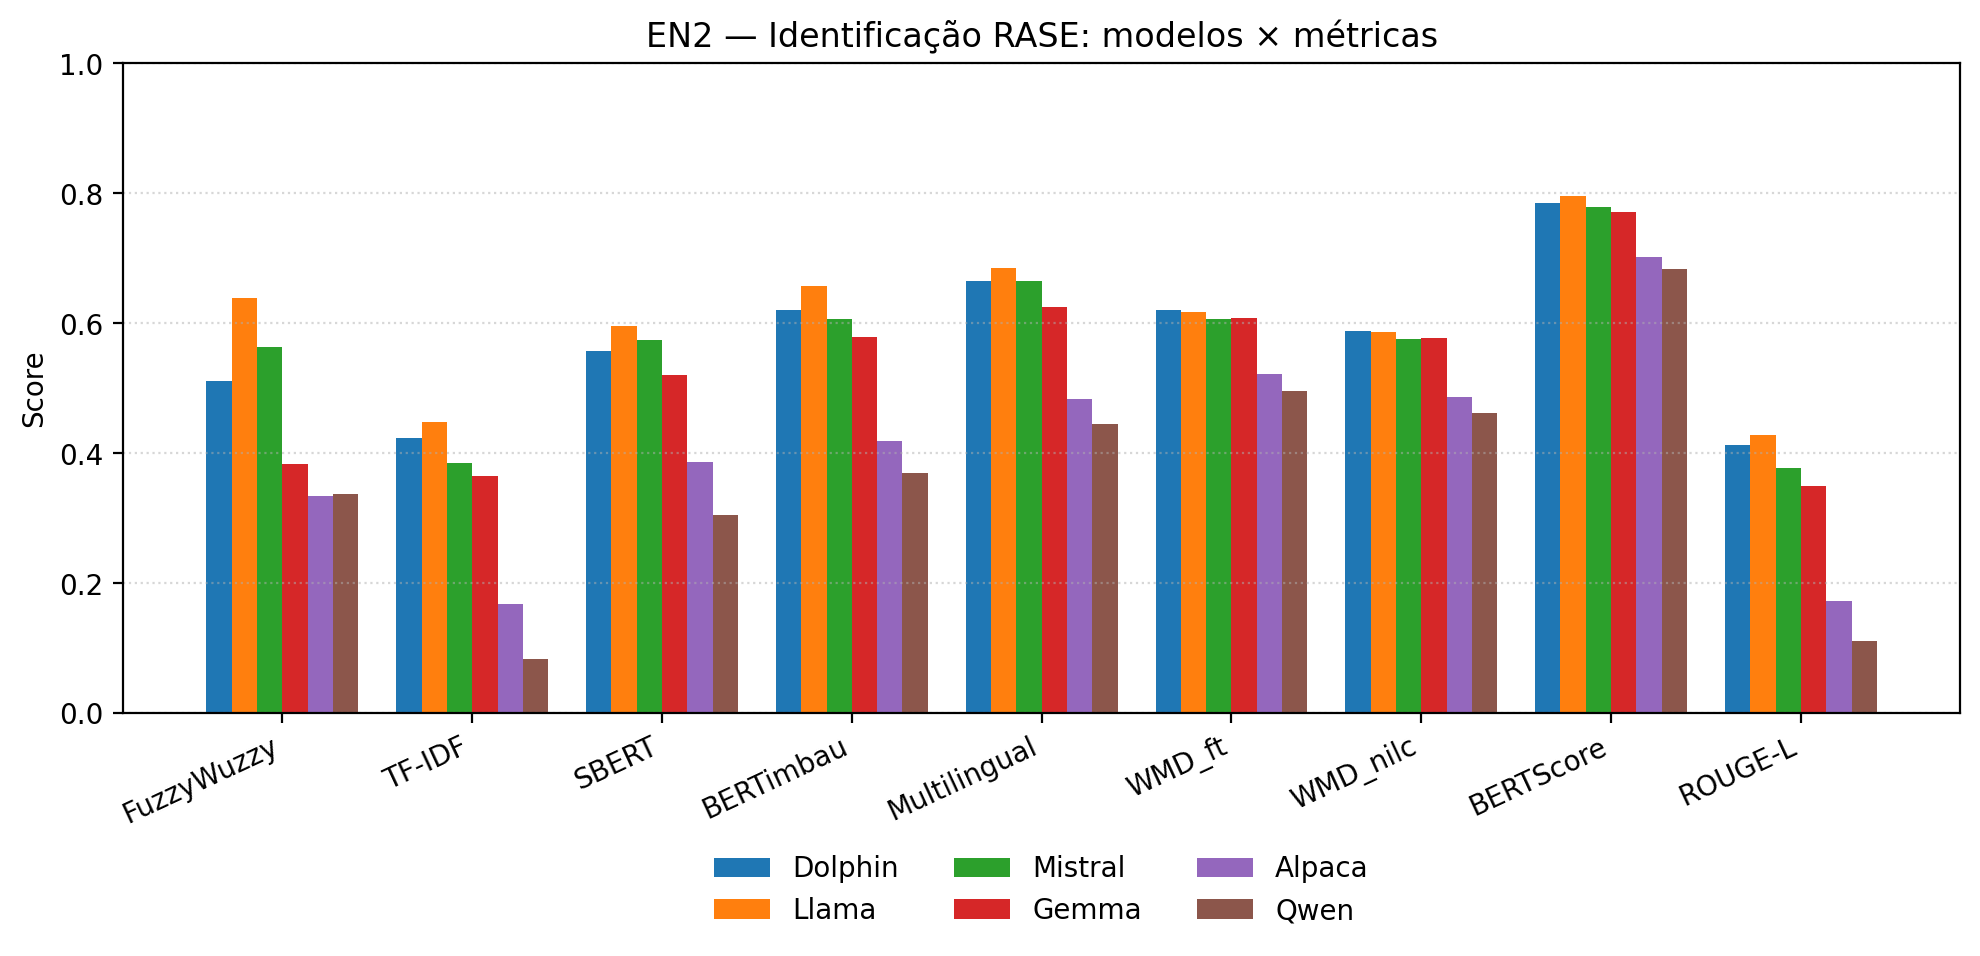
\includegraphics[width=0.95\linewidth]{Imagens/4.2.2-resultados-en2-barras.png}
\caption{Comparativo modelo $\times$ métrica em EN2.}
\label{img:4.2.2}
\end{figure}

\subsection{EN1N2 --- Pipeline Encadeado}

O EN1N2 testou a robustez do \textit{pipeline} totalmente automatizado: o N1 produzido pelo modelo na primeira etapa alimenta o N2 do mesmo modelo. Os resultados confirmam a hipótese de \textbf{propagação de erros}, mas com uma surpresa. As médias caem em relação ao EN2 em parte das métricas e se mantêm próximas ou até melhoram em outras --- caso das semânticas: Multilingual sobe de 0{,}595 para 0{,}679; BERTimbau de 0{,}542 para 0{,}631; SBERT de 0{,}490 para 0{,}594. O motivo é que o \textit{pipeline} produz saídas mais próximas das frases originais e, por isso, mais alinhadas ao texto de referência no nível semântico, ainda que perca precisão na atribuição dos operadores. A liderança é compartilhada: o \textbf{Dolphin} domina TF-IDF, WMD\_ft, WMD\_nilc, BERTScore e ROUGE-L; o \textbf{Llama} lidera SBERT e empata em Multilingual. Os números completos estão na Tabela~\ref{tab:resultados_en1n2}.

\begin{table}[ht]
\centering
\caption{Resultados por modelo em EN1N2 (similaridade).}
\label{tab:resultados_en1n2}
\scriptsize
\begin{tabular}{lccccccccc}
\hline
Modelo & FW & TF-IDF & SBERT & BERTimbau & Multi. & WMD\_ft & WMD\_nilc & BERTScore & ROUGE-L \\
\hline
Alpaca  & 0{,}375 & 0{,}285 & 0{,}494 & 0{,}523 & 0{,}581 & 0{,}573 & 0{,}538 & 0{,}742 & 0{,}282 \\
Dolphin & 0{,}549 & \textbf{0{,}529} & 0{,}662 & 0{,}711 & \textbf{0{,}749} & \textbf{0{,}673} & \textbf{0{,}644} & \textbf{0{,}826} & \textbf{0{,}509} \\
Gemma   & 0{,}391 & 0{,}458 & 0{,}615 & 0{,}656 & 0{,}701 & 0{,}646 & 0{,}617 & 0{,}804 & 0{,}436 \\
Llama   & \textbf{0{,}570} & 0{,}521 & \textbf{0{,}677} & \textbf{0{,}721} & \textbf{0{,}749} & 0{,}649 & 0{,}620 & 0{,}821 & 0{,}488 \\
Mistral & 0{,}559 & 0{,}489 & 0{,}667 & 0{,}698 & 0{,}740 & 0{,}648 & 0{,}618 & 0{,}817 & 0{,}468 \\
Qwen    & 0{,}342 & 0{,}219 & 0{,}448 & 0{,}478 & 0{,}551 & 0{,}562 & 0{,}530 & 0{,}731 & 0{,}240 \\
\hline
\end{tabular}
\end{table}

A Figura~\ref{img:4.2.3} apresenta o comparativo visual em EN1N2, evidenciando a alternância de liderança entre Dolphin e Llama por métrica.

\begin{figure}[ht]
\centering
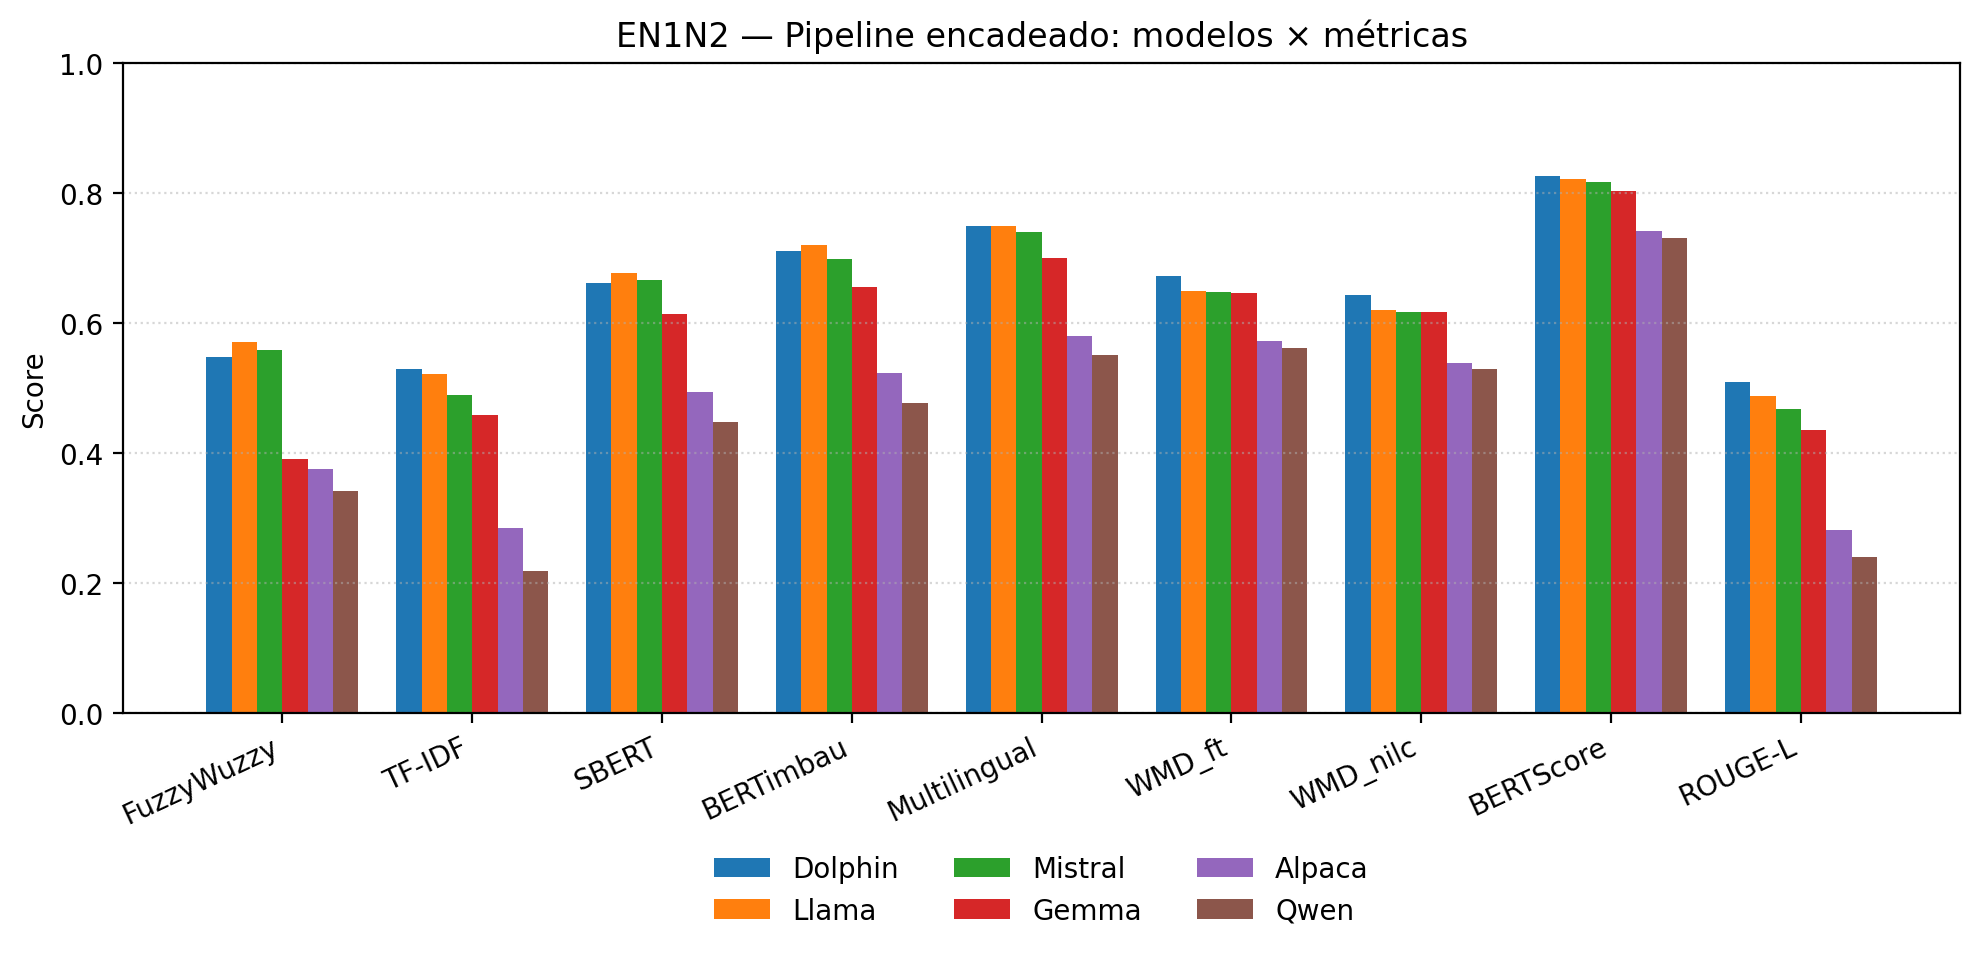
\includegraphics[width=0.95\linewidth]{Imagens/4.2.3-resultados-en1n2-barras.png}
\caption{Comparativo modelo $\times$ métrica em EN1N2.}
\label{img:4.2.3}
\end{figure}

\section{Resultados Isolados do Nível N3}
\label{sec:n3}

O N3 (estruturação semântica em JSON) também foi avaliado em isolamento, recebendo como entrada os operadores N2 de referência. Como a saída é \textit{quase-estruturada} e composta por campos curtos com vocabulário restrito (\texttt{object}, \texttt{property}, \texttt{comparation}, \texttt{target}, \texttt{unit}), as métricas de similaridade textual sobem para patamares bem mais altos do que em N1 e N2 --- ver Tabela~\ref{tab:resultados_n3}. As métricas de classificação por correspondência exata, em compensação, mostram um quadro bem mais duro: a precisão macro fica abaixo de 4\%. Isso sinaliza que os modelos preservam o significado, mas variam o vocabulário em relação à referência --- por exemplo, \texttt{target = ``público''} em vez de \texttt{target = ``uso público''}.

\begin{table}[ht]
\centering
\caption{Resultados por modelo em N3 isolado.}
\label{tab:resultados_n3}
\scriptsize
\begin{tabular}{lccccccccc}
\hline
Modelo & FW & TF-IDF & SBERT & BERTimbau & Multi. & WMD\_ft & WMD\_nilc & BERTScore & ROUGE-L \\
\hline
Alpaca  & 0{,}729 & 0{,}395 & 0{,}846 & 0{,}745 & 0{,}798 & 0{,}756 & 0{,}751 & 0{,}815 & 0{,}624 \\
Dolphin & 0{,}860 & 0{,}694 & 0{,}912 & 0{,}848 & 0{,}887 & 0{,}842 & 0{,}839 & 0{,}901 & 0{,}799 \\
Gemma   & 0{,}751 & 0{,}480 & 0{,}858 & 0{,}755 & 0{,}823 & 0{,}762 & 0{,}757 & 0{,}810 & 0{,}652 \\
Llama   & \textbf{0{,}892} & \textbf{0{,}736} & \textbf{0{,}947} & \textbf{0{,}897} & \textbf{0{,}928} & \textbf{0{,}915} & \textbf{0{,}912} & \textbf{0{,}925} & \textbf{0{,}871} \\
Mistral & 0{,}877 & 0{,}689 & 0{,}938 & 0{,}891 & 0{,}914 & 0{,}903 & 0{,}900 & 0{,}922 & 0{,}842 \\
Qwen    & 0{,}872 & 0{,}590 & 0{,}937 & 0{,}877 & 0{,}889 & 0{,}898 & 0{,}895 & 0{,}905 & 0{,}804 \\
\hline
\multicolumn{10}{c}{Métricas de classificação macro por campo (Acurácia / Precisão / Revocação / F1)} \\
\hline
Alpaca  & \multicolumn{9}{l}{0{,}283 / 0{,}012 / 0{,}434 / 0{,}024} \\
Dolphin & \multicolumn{9}{l}{0{,}705 / 0{,}034 / 0{,}447 / 0{,}062} \\
Gemma   & \multicolumn{9}{l}{0{,}292 / 0{,}017 / \textbf{0{,}603} / 0{,}033} \\
Llama   & \multicolumn{9}{l}{0{,}725 / \textbf{0{,}038} / 0{,}361 / \textbf{0{,}067}} \\
Mistral & \multicolumn{9}{l}{\textbf{0{,}760} / 0{,}037 / 0{,}371 / 0{,}066} \\
Qwen    & \multicolumn{9}{l}{0{,}692 / 0{,}004 / 0{,}063 / 0{,}008} \\
\hline
\end{tabular}
\end{table}

\subsection{EN3 --- Estruturação Semântica em JSON}

O EN3 mede a etapa de tradução dos operadores RASE para JSON estruturado, alimentando o N3 com o N2 de referência do \textit{dataset}. Aqui a comparação não é entre \textit{strings} normativas inteiras, e sim campo a campo --- \texttt{type}, \texttt{object}, \texttt{property}, \texttt{comparation}, \texttt{target} e \texttt{unit} ---, entre a saída do modelo e o JSON anotado. As mesmas métricas de similaridade dos outros experimentos rodam sobre a serialização canônica dos campos, somadas às métricas de classificação --- e, neste caso, \textit{verdadeiro positivo} exige correspondência exata por campo.

O setup foi idêntico ao dos experimentos anteriores: os mesmos seis LLMs servidos via Ollama, os mesmos \textit{prompts} \textit{few-shot} por operador, o mesmo \textit{dataset} de 79 normas. Saídas por modelo ficam em arquivos JSON dedicados (\texttt{generate\_n3\_llama.json}, por exemplo); o agregado vive em um único arquivo de métricas (\texttt{validate\_n3.json}), com a mesma estrutura de \textit{averages} usada nos outros experimentos. As tendências por família de métrica seguem o que se viu em EN2: semânticas acima das lexicais, e TF-IDF e FuzzyWuzzy mais sensíveis a variação de superfície no JSON. A correspondência exata por campo é mais dura que o limiar de similaridade adotado em N1 e N2, o que derruba a precisão observada --- em especial nos modelos com menor aderência ao esquema (Alpaca e Qwen).

\subsection{EN1N2N3 --- Pipeline Encadeado Completo}

O EN1N2N3 é o \textit{pipeline} automatizado de ponta a ponta: o N1 gerado alimenta o N2 do mesmo modelo, e o N2 gerado alimenta o N3 do mesmo modelo. Este é o cenário que replica o uso real em produção --- a única entrada é o texto bruto da norma, e a saída final é o JSON estruturado por operador. Como cada etapa acumula transformações, é também o experimento mais sujeito à \textbf{propagação de erros}: as médias ficam abaixo das observadas em EN3 e em EN1N2.

A saída de cada modelo é persistida em um arquivo JSON próprio (\texttt{generate\_n1n2n3\_llama.json}, por exemplo), e as métricas agregadas ficam em um arquivo único do experimento (\texttt{validate\_n1n2n3.json}), com a mesma estrutura de campos dos demais. Em linha com o padrão observado em EN1N2, os modelos com melhor desempenho semântico isolado (Llama e Dolphin) preservam vantagem relativa também na cadeia completa --- já Alpaca e Qwen acumulam queda em todas as métricas e entregam o pior desempenho global.

\section{Resultados por Modelo}

A Tabela~\ref{tab:ranking_global} traz a média global por modelo, agregando as nove métricas de similaridade textual sobre os três experimentos (EN1, EN2 e EN1N2). O ranking final foge do esperado: o líder é o \textbf{Dolphin}, não o Llama. A vantagem se sustenta na dominância quase total em EN1 e em um desempenho competitivo nas demais etapas. O Llama lidera em EN2 e fica entre os melhores no EN1N2 nas métricas semânticas. Mistral é o terceiro, seguido por Gemma, Alpaca e Qwen.

\begin{table}[ht]
\centering
\caption{Média global por modelo (nove métricas de similaridade $\times$ três experimentos).}
\label{tab:ranking_global}
\begin{tabular}{lcccc}
\hline
Modelo  & EN1   & EN2   & EN1N2 & Média Global \\
\hline
Dolphin & 0{,}801 & 0{,}576 & 0{,}650 & \textbf{0{,}676} \\
Llama   & 0{,}724 & 0{,}605 & 0{,}646 & 0{,}658 \\
Mistral & 0{,}757 & 0{,}570 & 0{,}634 & 0{,}654 \\
Gemma   & 0{,}738 & 0{,}531 & 0{,}591 & 0{,}620 \\
Alpaca  & 0{,}676 & 0{,}408 & 0{,}488 & 0{,}524 \\
Qwen    & 0{,}602 & 0{,}366 & 0{,}456 & 0{,}475 \\
\hline
\end{tabular}
\end{table}

A Figura~\ref{img:4.3.1} apresenta a mesma informação em forma de \textit{heatmap}, evidenciando visualmente as zonas de queda de desempenho entre EN1 e EN2 e o destaque do Dolphin em EN1.

\begin{figure}[ht]
\centering
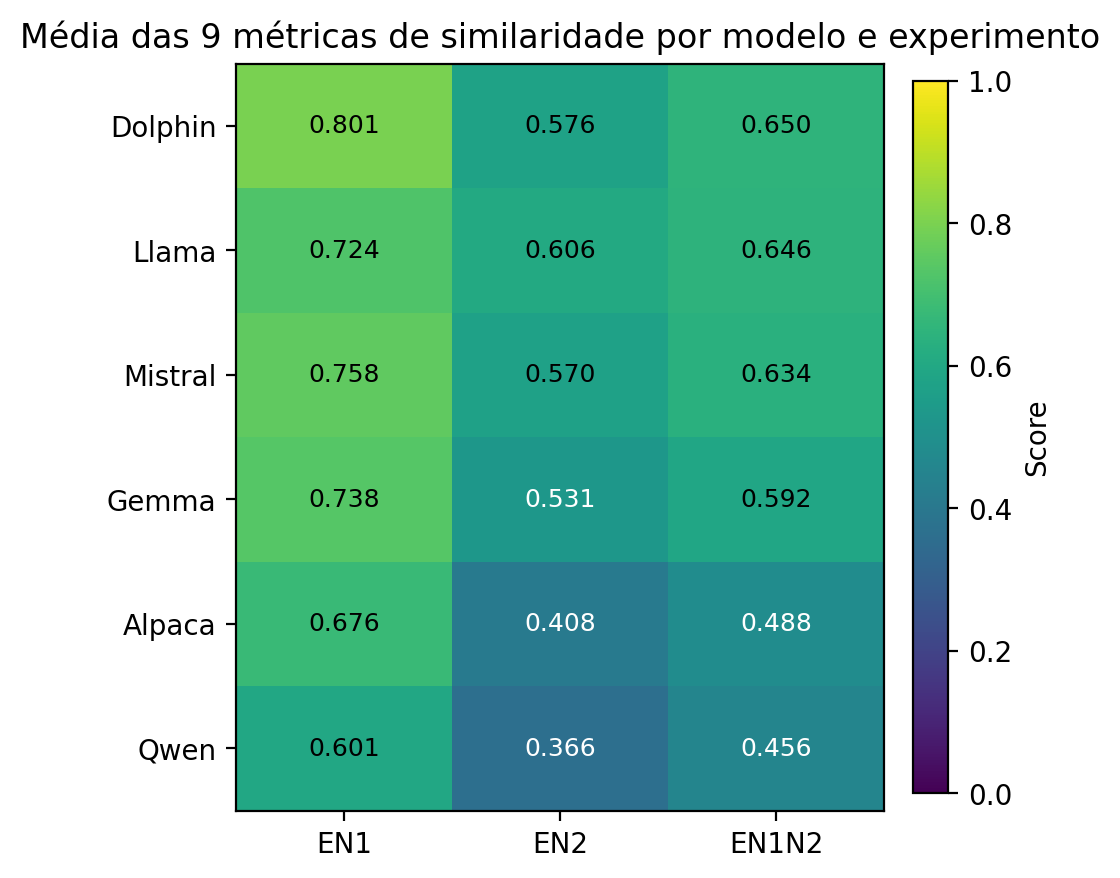
\includegraphics[width=0.7\linewidth]{Imagens/4.3.1-heatmap-global.png}
\caption{Heatmap das médias por modelo e experimento (média das nove métricas de similaridade).}
\label{img:4.3.1}
\end{figure}

A seguir, destacam-se as observações por modelo.

\textbf{Dolphin.} Foi o melhor segmentador em EN1, com domínio absoluto nas nove métricas (BERTimbau~0{,}891; Multilingual~0{,}913; SBERT~0{,}873; BERTScore~0{,}905) e a melhor F1 macro de classificação no experimento (0{,}806). No EN2, liderou em WMD\_ft (0{,}620), WMD\_nilc (0{,}589) e F1 macro (0{,}286). No EN1N2, ficou à frente em TF-IDF (0{,}529), WMD\_ft (0{,}673), WMD\_nilc (0{,}644), BERTScore (0{,}826) e ROUGE-L (0{,}509). Soma-se a isso o baixo custo computacional (Seção~\ref{sec:tempo}), o que rende a melhor relação custo-benefício observada.

\textbf{Llama.} Foi o melhor em EN2 em sete métricas --- FuzzyWuzzy (0{,}638), TF-IDF (0{,}447), SBERT (0{,}595), BERTimbau (0{,}657), Multilingual (0{,}685), BERTScore (0{,}796) e ROUGE-L (0{,}427) ---, além da maior acurácia macro de classificação no mesmo experimento (0{,}439). No EN1N2, liderou em FuzzyWuzzy (0{,}570), SBERT (0{,}677) e BERTimbau (0{,}721), empatando com o Dolphin em Multilingual (0{,}749). No N3 isolado, foi o melhor em todas as métricas de similaridade textual.

\textbf{Mistral.} Desempenho consistente em todos os cenários. Ficou próximo dos líderes em EN1 (Multilingual~0{,}899; BERTimbau~0{,}874) e em EN1N2 (Multilingual~0{,}740; BERTimbau~0{,}698), e entregou a segunda melhor acurácia macro do EN2 (0{,}434).

\textbf{Gemma.} Aparece como líder em revocação macro de classificação tanto no EN1 (0{,}917) quanto no EN2 (0{,}300) --- ou seja, boa cobertura, com precisão menor. As médias semânticas ficam em patamar intermediário.

\textbf{Alpaca.} Desempenho fraco em todos os experimentos, com queda acentuada no EN2 (SBERT~0{,}386; F1 macro~0{,}105).

\textbf{Qwen.} Pior desempenho geral. Colapsou no EN2 (TF-IDF~0{,}083; F1 macro~0{,}044) e teve a maior latência do \textit{pipeline} encadeado (ver Seção~\ref{sec:tempo}). Pesa também a tendência do modelo a gerar saídas em chinês simplificado, fora do idioma esperado.

\section{Análise por Métrica}

\textbf{Métricas lexicais.} FuzzyWuzzy e TF-IDF caem claramente de EN1 para EN2 (FuzzyWuzzy: 0{,}475 $\rightarrow$ 0{,}461; TF-IDF: 0{,}636 $\rightarrow$ 0{,}312). Como dependem de sobreposição lexical, essas métricas punem as reformulações sintáticas e as sinonímias geradas pelos LLMs.

\textbf{Métricas semânticas.} SBERT, BERTimbau e Multilingual mantêm médias altas e estáveis. O BERTimbau, treinado sobre texto jurídico em português, fica ligeiramente acima do SBERT em quase todos os modelos e experimentos (EN1: 0{,}816 \textit{vs.}~0{,}801; EN1N2: 0{,}631 \textit{vs.}~0{,}594) --- evidência prática do ganho de usar \textit{embeddings} de domínio para validar transformações normativas.

\textbf{Métricas voltadas para geração.} O BERTScore teve a maior média absoluta em EN2 (0{,}753) e em EN1N2 (0{,}790), graças ao alinhamento ótimo entre \textit{tokens} mesmo quando há forte reformulação. Já o ROUGE-L comportou-se como métrica lexical, com queda acentuada em EN2 (0{,}308).

\textbf{Métricas de distância (WMD).} Desempenho intermediário, entre lexicais e semânticas. Os valores foram mais altos em EN1 (WMD\_ft~0{,}716; WMD\_nilc~0{,}688), refletindo a proximidade lexical maior entre as saídas de segmentação e o texto original.

\textbf{Métricas de classificação.} Em EN1, a F1 macro chega a 0{,}806 (Dolphin), o que indica que a maior parte das sentenças atômicas é segmentada corretamente. Em EN2, a F1 desaba para 0{,}286 no melhor caso (Dolphin), com colapso em Seleção e Exceção --- F1 próxima de zero para todos os modelos. Esses dois operadores são especialmente difíceis de identificar mesmo para os líderes. Em N3, a baixa precisão por correspondência exata mostra que o emparelhamento \textit{token} a \textit{token} é severo demais para um campo cuja semântica resiste a variações léxicas legítimas.

As Figuras~\ref{img:4.4.1}, \ref{img:4.4.2} e \ref{img:4.4.3} apresentam o mapa de calor modelo $\times$ métrica em cada experimento, com os valores numéricos sobrepostos.

\begin{figure}[ht]
\centering
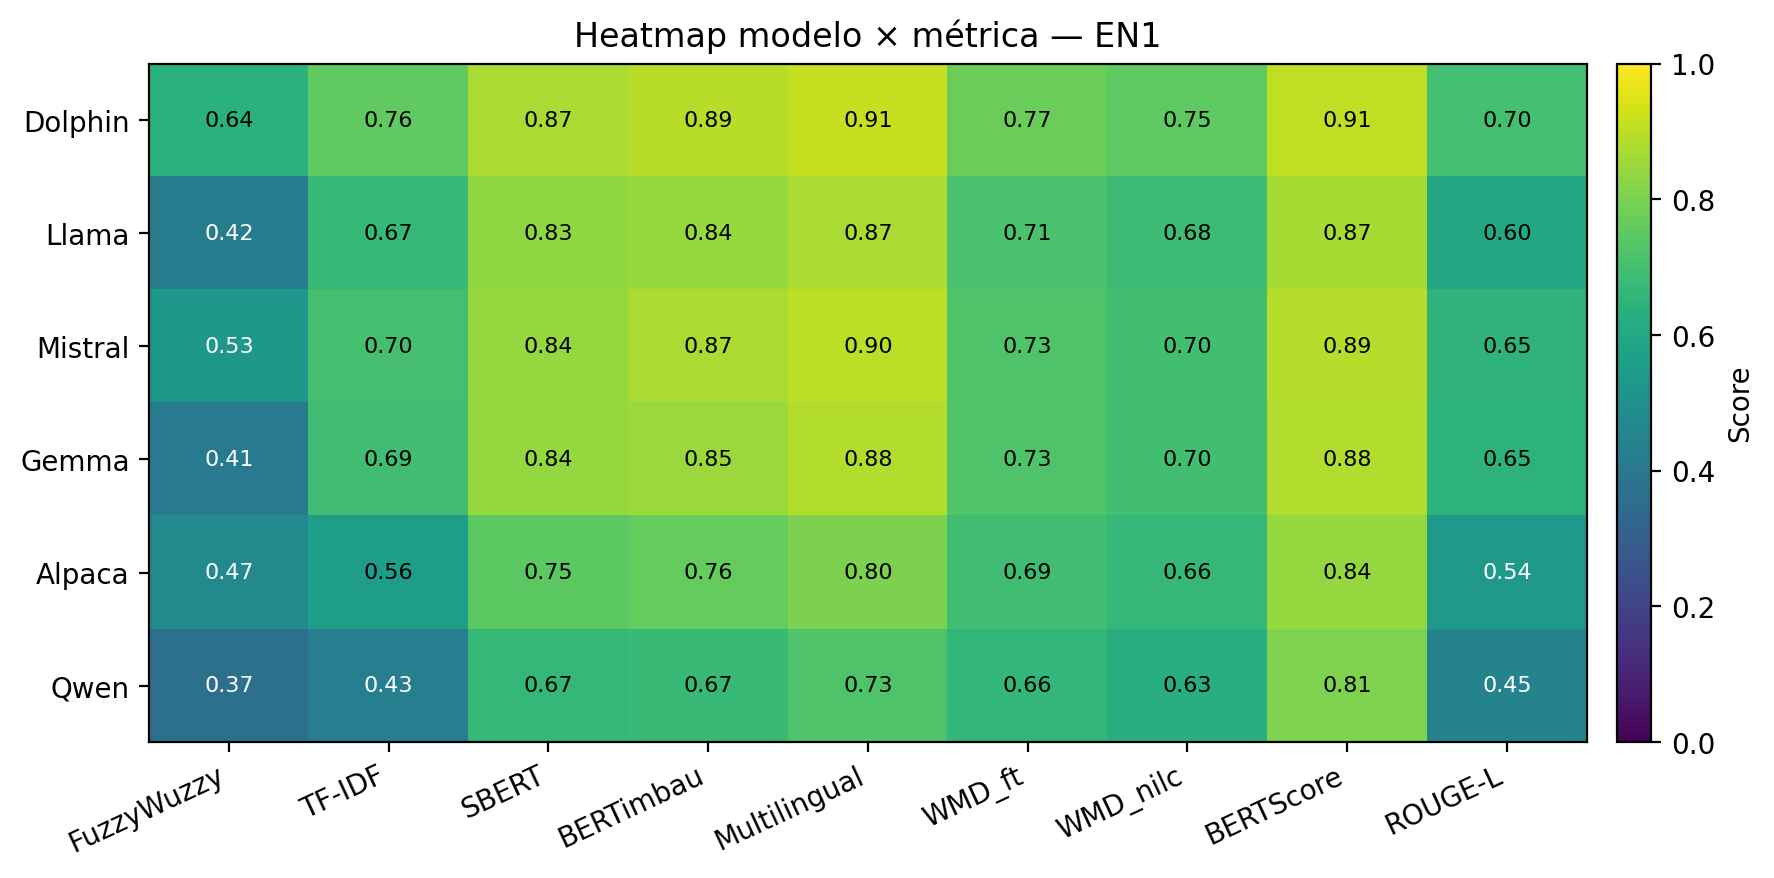
\includegraphics[width=0.9\linewidth]{Imagens/4.4.1-heatmap-en1.png}
\caption{Heatmap modelo $\times$ métrica em EN1.}
\label{img:4.4.1}
\end{figure}

\begin{figure}[ht]
\centering
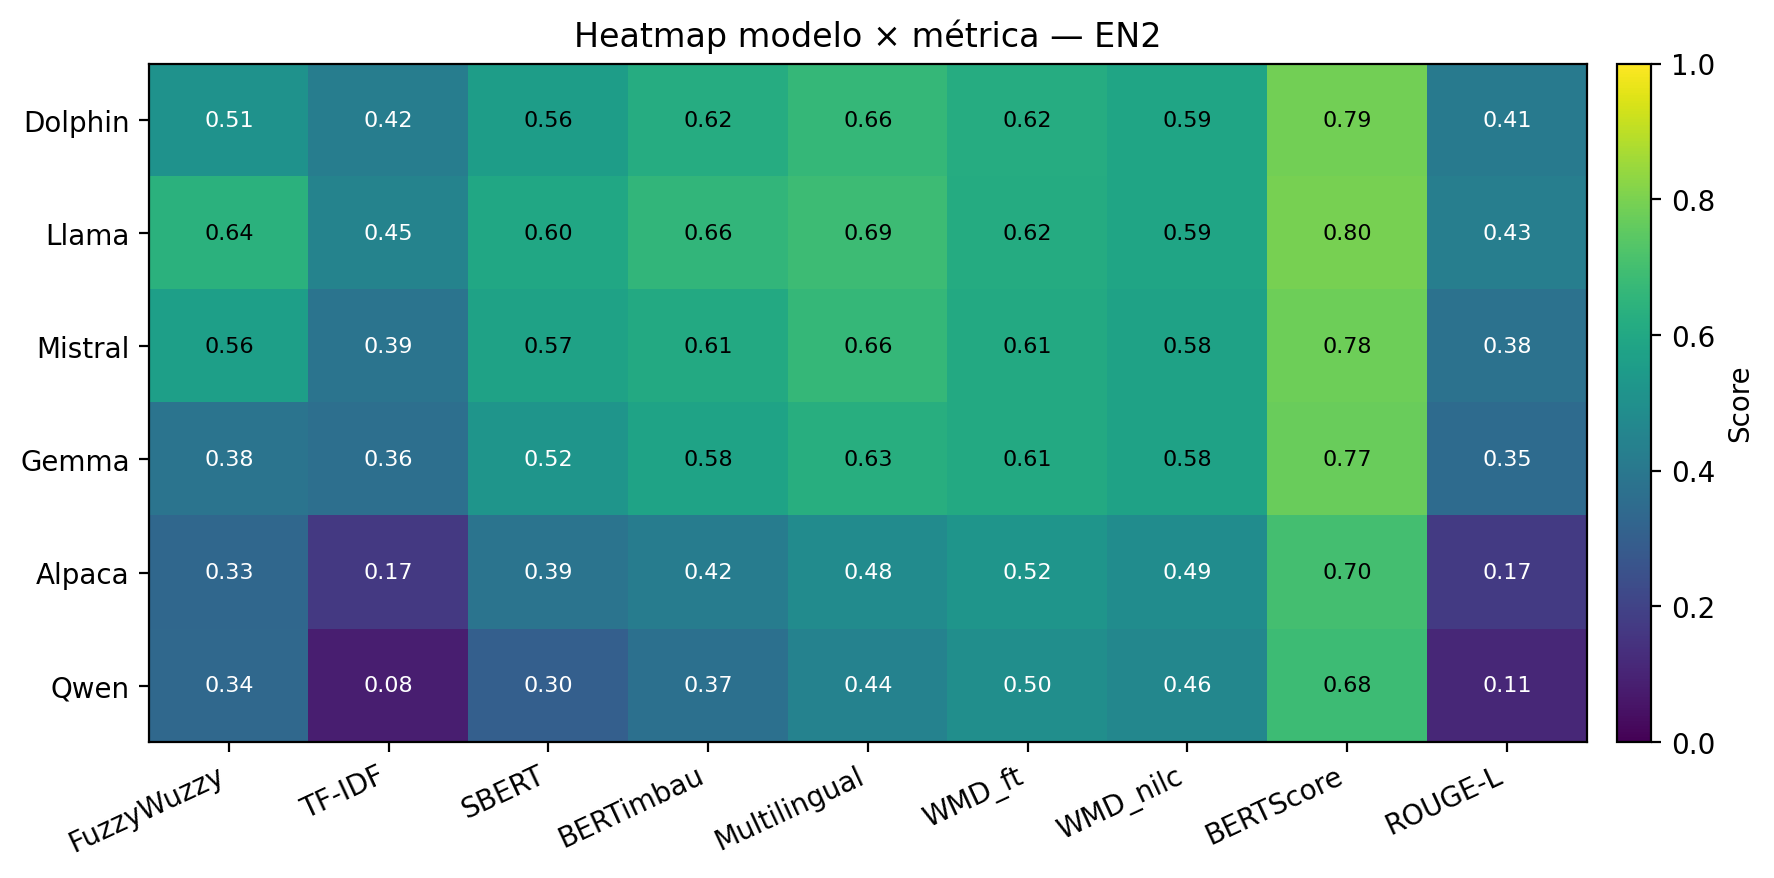
\includegraphics[width=0.9\linewidth]{Imagens/4.4.2-heatmap-en2.png}
\caption{Heatmap modelo $\times$ métrica em EN2.}
\label{img:4.4.2}
\end{figure}

\begin{figure}[ht]
\centering
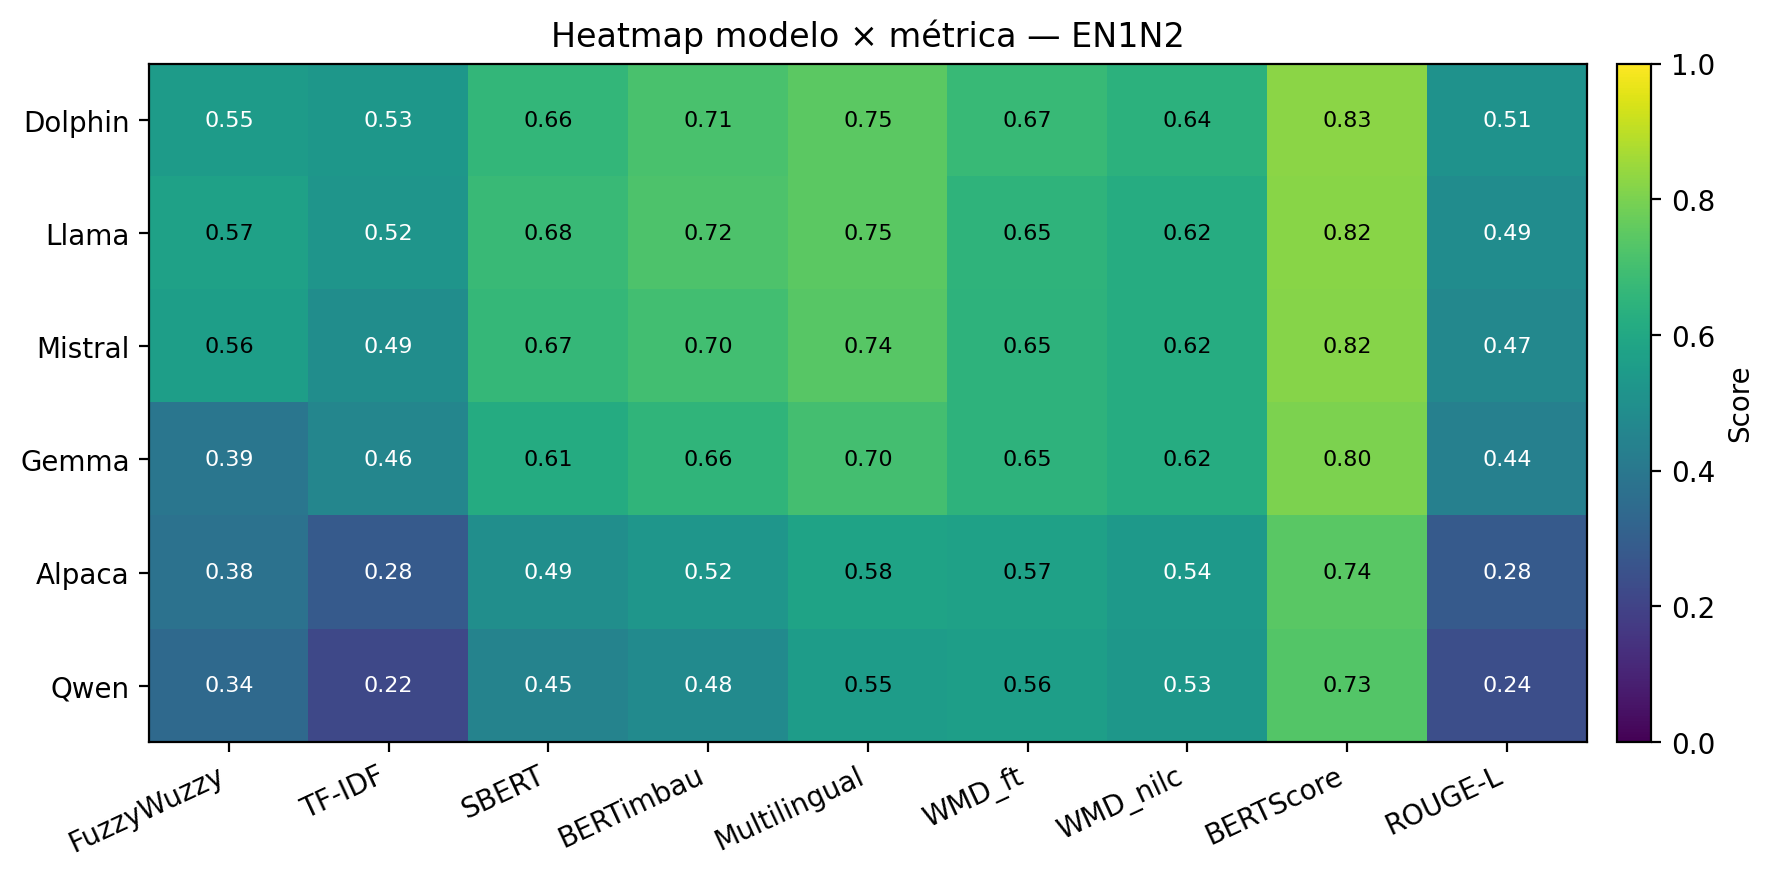
\includegraphics[width=0.9\linewidth]{Imagens/4.4.3-heatmap-en1n2.png}
\caption{Heatmap modelo $\times$ métrica em EN1N2.}
\label{img:4.4.3}
\end{figure}

\section{Tempo de Execução}
\label{sec:tempo}

O tempo total de geração foi medido por modelo e por nível. A Tabela~\ref{tab:tempo_n1} traz os tempos em N1; a Tabela~\ref{tab:tempo_n2}, em N2; e a Tabela~\ref{tab:tempo_n1n2}, no \textit{pipeline} encadeado N1N2. Os tempos da etapa N3 ficam no campo \texttt{time} dos arquivos JSON de geração e seguem o padrão das demais etapas: Llama como modelo mais oneroso, Dolphin como o mais econômico em qualidade equivalente.

\begin{table}[ht]
\centering
\caption{Tempo total de geração por modelo em N1.}
\label{tab:tempo_n1}
\begin{tabular}{lrr}
\hline
Modelo & Tempo (s) & Tempo (h:mm:ss) \\
\hline
Alpaca  & 104{,}55     & 0:01:44 \\
Dolphin & 62{,}65      & 0:01:02 \\
Gemma   & 133{,}04     & 0:02:13 \\
Llama   & 5\,676{,}97  & 1:34:36 \\
Mistral & 70{,}04      & 0:01:10 \\
Qwen    & 309{,}59     & 0:05:09 \\
\hline
\end{tabular}
\end{table}

\begin{table}[ht]
\centering
\caption{Tempo total de geração por modelo em N2.}
\label{tab:tempo_n2}
\begin{tabular}{lrr}
\hline
Modelo & Tempo (s) & Tempo (h:mm:ss) \\
\hline
Alpaca  & 249{,}10     & 0:04:09 \\
Dolphin & 124{,}69     & 0:02:04 \\
Gemma   & 244{,}19     & 0:04:04 \\
Llama   & 6\,895{,}71  & 1:54:55 \\
Mistral & 123{,}63     & 0:02:03 \\
Qwen    & 6\,515{,}09  & 1:48:35 \\
\hline
\end{tabular}
\end{table}

\begin{table}[ht]
\centering
\caption{Tempo total de geração por modelo em N1N2.}
\label{tab:tempo_n1n2}
\begin{tabular}{lrr}
\hline
Modelo & Tempo (s) & Tempo (h:mm:ss) \\
\hline
Alpaca  & 330{,}84      & 0:05:30 \\
Dolphin & 104{,}28      & 0:01:44 \\
Gemma   & 427{,}22      & 0:07:07 \\
Llama   & 9\,450{,}14   & 2:37:30 \\
Mistral & 138{,}39      & 0:02:18 \\
Qwen    & 10\,093{,}84  & 2:48:13 \\
\hline
\end{tabular}
\end{table}

Os tempos expõem um \textit{trade-off} nítido entre qualidade e custo computacional. Llama e Qwen são os mais lentos --- respectivamente 1h34min e 5min em N1; 2h37min e 2h48min em N1N2. O Dolphin combina a melhor média global de qualidade com tempos na casa de 1 a 2 minutos (62~s em N1; 1m44s em N1N2), o que o coloca como \textbf{cerca de 90 vezes mais rápido que o Llama} no \textit{pipeline} encadeado, com qualidade equivalente ou superior em várias métricas. Mistral fica em situação parecida: tempos curtos (em torno de 2 minutos) e qualidade próxima da liderança.

\section{Discussão Integrada}

A leitura conjunta dos três experimentos e das treze métricas permite consolidar cinco observações.

\textbf{1. \textit{Embeddings} semânticos e BERTScore são as métricas mais adequadas a esta tarefa.} SBERT, BERTimbau, Multilingual e BERTScore capturam equivalência mesmo quando há reformulação lexical pesada, e são as métricas mais estáveis ao longo dos experimentos. O BERTimbau, treinado em corpus jurídico em PT-BR, fica ligeiramente acima do SBERT --- evidência do ganho de \textit{embeddings} de domínio.

\textbf{2. O \textit{pipeline} encadeado não degrada todas as métricas de forma uniforme.} A queda esperada pela propagação de erros aparece nas lexicais (FuzzyWuzzy, TF-IDF e ROUGE-L). Já nas semânticas, o EN1N2 chega a \textit{superar} o EN2 isolado nas médias agregadas (Multilingual~0{,}679 \textit{vs.}~0{,}595): o N1 produzido pelo próprio modelo tende a gerar frases próximas das originais, o que favorece o emparelhamento semântico, mesmo quando o N2 erra na atribuição dos operadores. As métricas de classificação confirmam, porém, que esse ganho não se converte em classificação RASE melhor --- o \textit{pipeline} continua dependendo de saída atomizada e corretamente rotulada para que a verificação automática faça sentido.

\textbf{3. Há perfis complementares entre os modelos líderes.} O Dolphin lidera a qualidade global (0{,}676) e entrega o melhor custo-benefício; domina o EN1 e fica à frente nas métricas de distância do EN1N2. O Llama lidera o EN2 e fica entre os melhores nas métricas semânticas do EN1N2 e no N3 isolado --- é a escolha quando se tolera o custo computacional.

\textbf{4. Qwen e Alpaca não são recomendados.} Ambos têm desempenho consistentemente inferior em todas as métricas e experimentos. O Qwen ainda registra a maior latência do \textit{pipeline} encadeado (2h48min) e tende a gerar saídas fora do idioma esperado.

\textbf{5. A decomposição em três níveis foi decisiva.} Separar segmentação (N1), classificação RASE (N2) e estruturação JSON (N3) viabilizou saídas válidas sem \textit{Fine-Tuning} nem \textit{Retrieval-Augmented Generation} --- ou seja, Engenharia de Prompt sozinha basta para alcançar similaridade semântica perto de 0{,}90 nos melhores cenários (Dolphin em EN1, com BERTimbau~0{,}891; Llama em N3 isolado, com SBERT~0{,}947). O que sobra de dificuldade está concentrado na classificação correta dos operadores Seleção e Exceção em N2 --- as classes mais difíceis para todos os modelos avaliados.
